% !TeX spellcheck = es_ES
\documentclass[a4paper, 11pt]{article}
\usepackage[table,xcdraw]{xcolor}
\usepackage{graphicx}
\usepackage{hyperref}
\usepackage{mathtools}
\usepackage{amsmath}
\usepackage[spanish, activeacute]{babel} %Definir idioma español
\usepackage[utf8]{inputenc} %Codificacion utf-8

\usepackage{geometry}
\geometry{left=2.5cm,right=2.5cm,top=2.5cm,bottom=2.5cm}

\DeclareMathOperator*{\argmax}{arg\,max}

\title{\Large{\textbf{Detección de caras basada en Redes Neuronales}}}

\author{\textit{Francisco Rubin Capalbo}\\
		Universidad Politécnica de Valencia }

\date{\today}

\begin{document}
    
    \maketitle
    \section{Introducción}
    	Este trabajo consiste en el diseño y la implementación de un detector de caras basado en redes neuronales. El detector se puede dividir en dos partes igual de importantes: el clasificador de caras y el extractor de crops a clasificar. \\
    \section{Dataset}
		El dataset necesario para entrenar el clasificador de caras consiste en un conjunto de imágenes que contienen una cara (centrada, con un pequeño margen) y otro conjunto igual de grande que no contiene ninguna. 
		
		\subsection{No-caras}
		Para obtener el conjunto de no-caras\cite{script-no-caras}, he empleado varias herramientas. Por un lado, he descargado imágenes en masa de una API de google imágenes. He utilizado keywords con una gran probabilidad de representar imágenes sin caras, como 'carretera', 'espacio', 'texturas', etc. \\
		
		 A continuación, he utilizado un detector de caras de OpenCV basado en filtros Haar, para descartar las imágenes contenedoras de una o más caras. De las imágenes resultantes he extraído crops de ancho y alto aleatorios en posiciones aleatorias. En total, el dataset de no-caras está compuesto por unas 150 mil imágenes. 
		 
		 \subsection{Caras}
		 Para el dataset de caras he utilizado CelebA\cite{celeb-a}. El problema de este dataset es que las caras que contiene no están centradas, y en algunas imágenes aparece el cuerpo entero. Para resolver este problema, he vuelto a recurrir a el detector de caras de OpenCV\cite{script-caras}, para detectar una cara por imagen y extraerla a un archivo a parte. En total, he conseguido unas 150 mil caras. 

		\subsection{Nota}
		Un detalle que me preocupa del método utilizado para obtener el dataset, es que depende completamente de el detector implementado en OpenCV con filtros Haar. Esto podría implicar que nuestro modelo no puede aprender de caras extrañas que los filtros Haar no detectan, así poniendo un techo a la precisión obtenida. Por otro lado, si los filtros Haar detectan caras dónde no las hay, éstas serán utilizadas incorrectamente en nuestro modelo. A pesar de esto, no he encontrado otra manera más efectiva de obtener el Dataset.
	\section{Clasificador}
		El objetivo del clasificador\cite{classifier-training} es decidir si la imagen que recibe como input es una cara o no. Es un clasificador binario (cara / no cara), por lo cual utilizamos la función de pérdida 'Binary Cross Entropy'.
		
		\subsection{Data Augmentation}
			Una manera muy efectiva de que el clasificador generalice mejor es haciendo data augmentation. Para este problema he aplicado rotación, traslación, escalado y flip horizontal de manera aleatoria. De especial importancia es la rotación, ya que la mayoría de las caras del dataset aparecen en posición vertical, y queremos que el clasificador sepa reconocer caras en cualquier orientación.
			
		\subsection{Normalización de datos}
			Todas las imágenes pasadas al clasificador son normalizadas de la misma manera. Primero se convierten a blanco y negro y se aplica una normalización de color (x - mean / std). Por último, se escalan a un tamaño de 24x24 píxeles.

		\subsection{Modelos}
			
	- diferentes modelos / arquitecturas
		- bce loss
		- descripciones modelos
		- resultados de cada uno de ellos (tabla)
			- mencionar que todas las pruebas fueron realizadas en un dataset pequeño, incluyendo sólo un 5\% de los datos
			
			
		\begin{table}[htb!]
			\centering
			\caption{Evaluación Modelos}
			\label{evaluacion-modelos}
			\begin{tabular}{|c|c|c|}
				\hline
				\textbf{Modelo}                                                 & \textbf{Accuracy} & \textbf{Tiempo (segundos)} \\ \hline
				Modelo 1                                                            & 99.766                & 0.316               \\ \hline
				Modelo 2                                                              & 99.732                & 0.295              \\ \hline
				Modelo 3                                                   & 99.465                & 0.277                \\ \hline
				\textbf{Modelo 4}                                                    & \textbf{99.699}             & \textbf{0.271}               \\ \hline
				Modelo 5                                                    & 99.532             & 0.293               \\ \hline
				Modelo 6                                                    & 99.766             & 0.393               \\ \hline
			\end{tabular}
		\end{table}
			
			
			\begin{figure}[htb!]
				\begin{minipage}{1\textwidth}
					\centering
					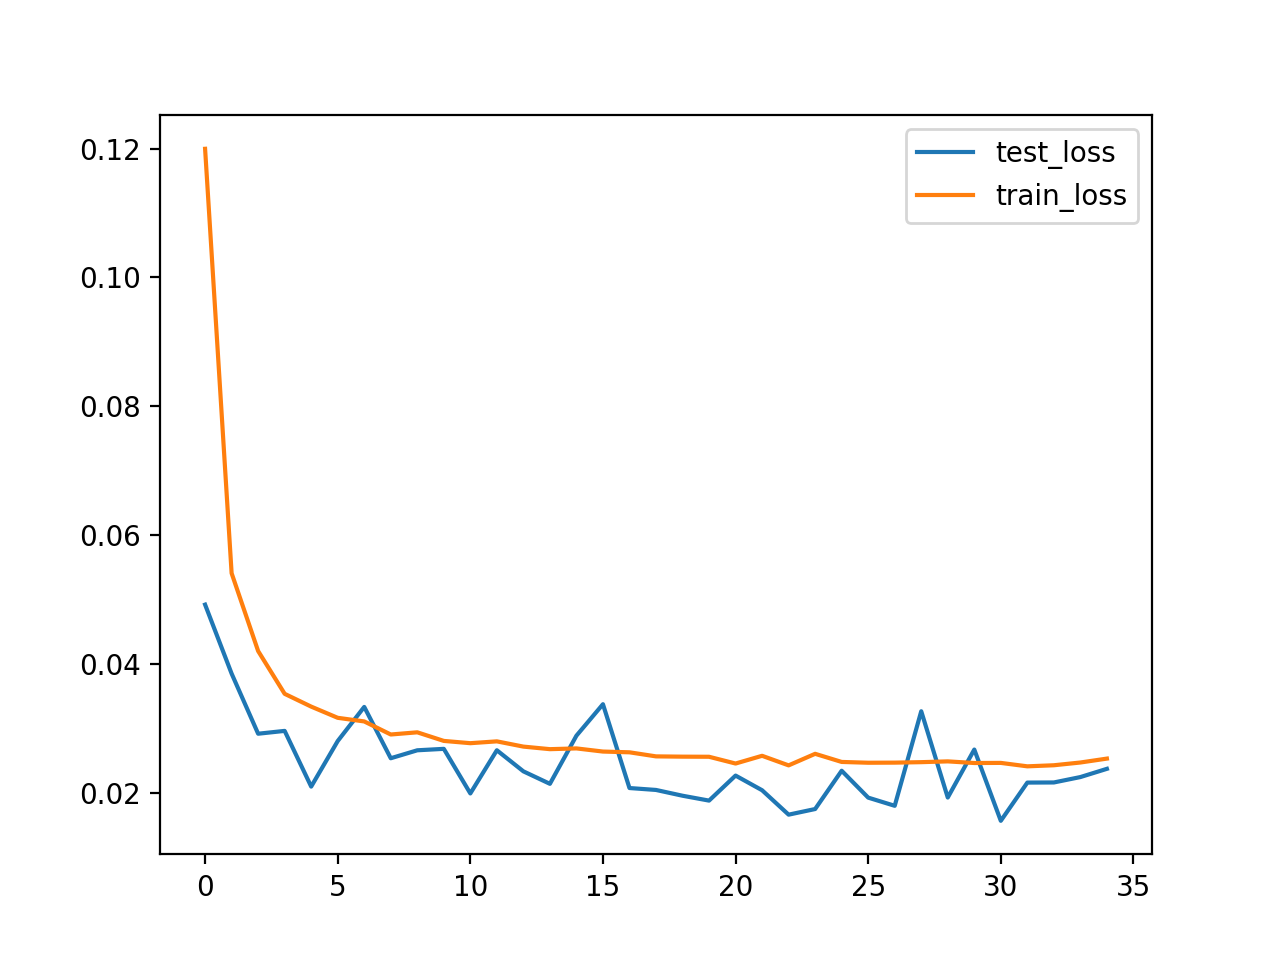
\includegraphics[scale=.5]{pics/model4_losses_per_epoch}
					\caption{Modelo 4: Loss por epoch}
					\label{fig:model4_losses_per_epoch}
				\end{minipage}\hfill
			\end{figure}
		
		
		\begin{figure}[htb!]
			\begin{minipage}{1\textwidth}
				\centering
				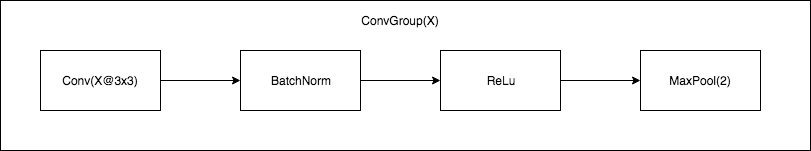
\includegraphics[scale=.5]{pics/convgroup}
			\end{minipage}\hfill
		\end{figure}
	

			\begin{figure}[htb!]
		\begin{minipage}{1\textwidth}
			\centering
			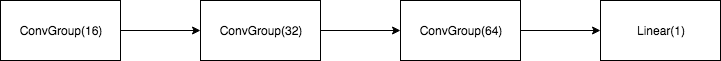
\includegraphics[scale=.5]{pics/model1}
					\caption{Modelo 1}
		\end{minipage}\hfill
	\end{figure}


		\begin{figure}[htb!]
	\begin{minipage}{1\textwidth}
		\centering
		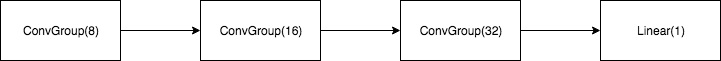
\includegraphics[scale=.5]{pics/model2}
				\caption{Modelo 2}
	\end{minipage}\hfill
\end{figure}


		\begin{figure}[htb!]
	\begin{minipage}{1\textwidth}
		\centering
		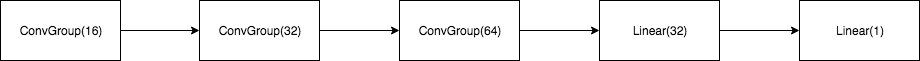
\includegraphics[scale=.5]{pics/model3}
		\caption{Modelo 3}
	\end{minipage}\hfill
\end{figure}


		\begin{figure}[htb!]
	\begin{minipage}{1\textwidth}
		\centering
		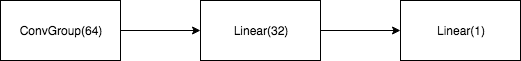
\includegraphics[scale=.5]{pics/model4}
				\caption{Modelo 4}
	\end{minipage}\hfill
\end{figure}		


		\begin{figure}[htb!]
	\begin{minipage}{1\textwidth}
		\centering
		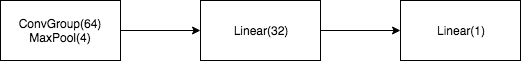
\includegraphics[scale=.5]{pics/model5}
				\caption{Modelo 5}
	\end{minipage}\hfill
\end{figure}


\begin{figure}[htb!]
	\begin{minipage}{1\textwidth}
		\centering
		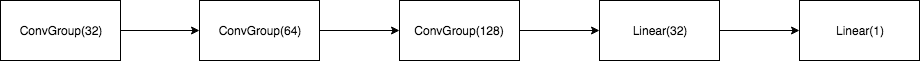
\includegraphics[scale=.5]{pics/model6}
				\caption{Modelo 6}
	\end{minipage}\hfill
\end{figure}	
			
- detector
	- downscale image to a max witdth and height to reduce number of crops
	- extracción de crops 
		- mencionar que al pasar los crops a memoria antes de clasificar mejoró de 180 segundos a 10 segundos
	- clasificación de crops en cara/no cara
	- pintar rectángulos en imagen final
	- tutorial de como usar el detector (para q lo pueda probar el profe)
- Trabajo futuro
	- user selective search para selección de crops
	- probar con depthwise separable convolutionals para mejorar velocidad
	- aumentar los saltos de zoom y translation para las seleccion de crops usando el modelo con data augmentation potenciada
	

\begin{thebibliography}{50}
	
	\bibitem{script-no-caras} 
	\href{https://github.com/pancho111203/pytorch-face-detection/blob/master/scripts/get_nofaces.py}{Script obtención no-caras}
	\bibitem{celeb-a} 
	\href{http://mmlab.ie.cuhk.edu.hk/projects/CelebA.html}{CelebA Dataset}
	\bibitem{script-caras} 
	\href{https://github.com/pancho111203/pytorch-face-detection/blob/master/scripts/crop_faces.py}{Script obtención caras}
	\bibitem{classifier-training} 
	\href{https://github.com/pancho111203/pytorch-face-detection/blob/master/face_classifier_training.py}{Entrenamiento clasificador}
	\bibitem{demo} 
	\href{url }{name}
	\bibitem{demo} 
	\href{url }{name}
	\bibitem{demo} 
	\href{url }{name}
	\bibitem{demo} 
	\href{url }{name}
	\bibitem{demo} 
	\href{url }{name}
	\bibitem{demo} 
	\href{url }{name}
\end{thebibliography}

\end{document}